\section{Theory}
	\subsection{Scattering Principle}
		When alpha-particles are allowed to collide with a thin gold foil in a process known as Rutherford Scattering, the pertubative potential of the colliding nucleus causes the particles to scatter or be deflected in various ways. The graphic below illustrates how most alpha-particle scattering occurs at angles smaller than one degree. However, a small number of particles exhibit significantly large scattering angles $(\theta)$, and in rare situations, they may even reverse their original direction at $180^\circ$ (back scattering). The only way to explain these early qualitative findings is to assume that the gold atoms have a very tiny nucleus that virtually contains the entire atomic mass and is positively charged. The nucleus was found in this manner.

		\begin{figure}[h]
			\centering
			\label{fig:1}
			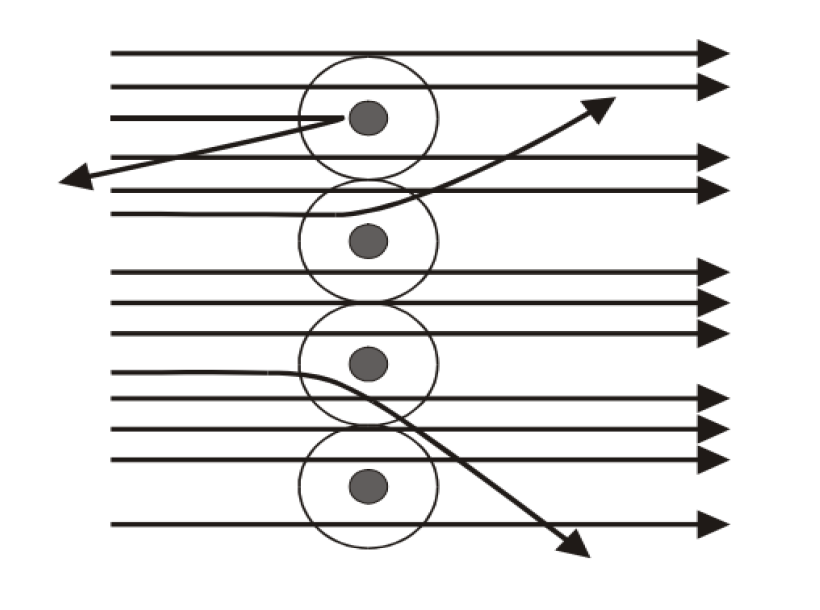
\includegraphics[width=0.8\columnwidth]{images/theory1.png}
			\caption{Scattering of alpha-particles by the nucleus}
		\end{figure}
	
	\subsection{Scattering Rate}
		The angular distribution of scattering rate is given by $N(\theta)$, and is equal to the number of particles scattered per unit time per unit solid angle. For a material with nuclear charge $Z$, the scattering rate for alpha particles $(Z = 2)$ emitted at a rate $N_0$ with energy $E_\alpha$ is given by:

		\begin{equation}
			\label{eq:1}
			N(\theta) = \frac{N_0c_FZ^2e^4d_F}{(8\pi\epsilon_0E_\alpha)^2\sin^4\frac{\theta}{2}}
		\end{equation}

		here $c_F$ is the atomic concentration in the foil and $d_F$ the thickness of the foil.

		The relevant shape of the scattering rate vs  angle graph is defined by the sine function, and is given by:

		$$f(\theta) = \frac{1}{\sin^4\frac{\theta}{2}}$$

		With increasing scattering angle theta, the values of $f(theta)$ rapidly decline, and there is a singularity at $\theta=0^\circ$. Higher scattering angles result in very tiny counting rates, hence in order to achieve an acceptable level of precision, the gate times $t(\theta)$ for calculating the counting rate $N(\theta)$ must be raised with rising angle theta. As a result, in the initial portion of the experiment, we begin at $5^\circ$ and gradually increase the gate duration as we climb higher until $30^\circ$.

		\subsubsection{Space Correction for Scattering Rate}

			The scattering rates $N_d(\theta)$ are determined by recording the pulse counts $n(\theta)$ for a given angle $\theta$ over a gate time t.

			$$N_d(\theta) = \frac{n(\theta)}{t}$$

			However, because to the clear design of the chamber utilised in this experiment, this $N_d(\theta)$ is for a flat scattering geometry. However, Rutherford's formula indicates that the theoretical function is connected to a three-dimensional geometry. The relationship between them is illustrated in the \hyperref[fig:2]{Figure 2}.

			\begin{figure}[h]
				\centering
				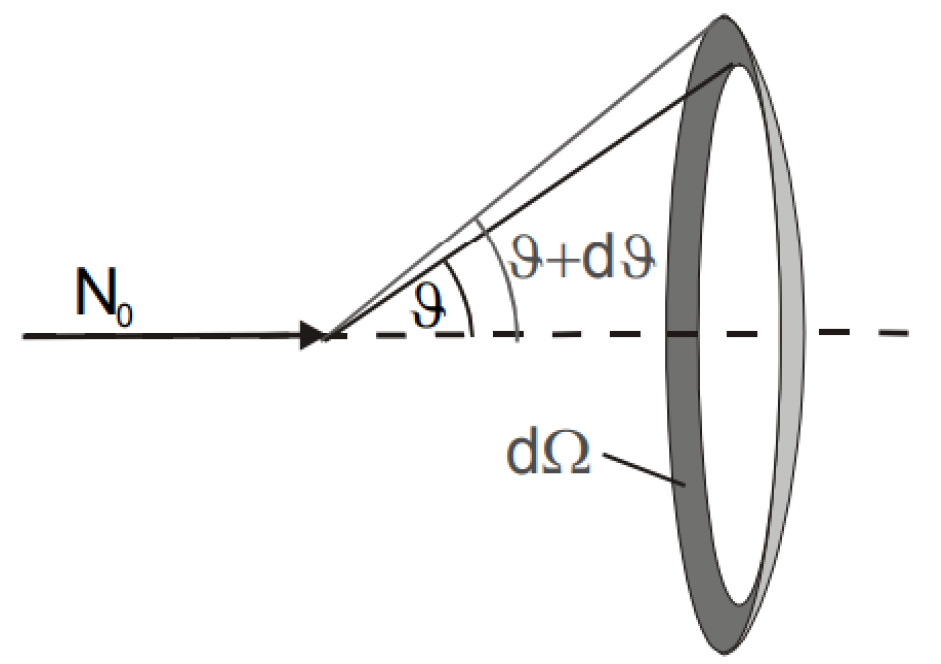
\includegraphics[width=0.8\columnwidth]{images/theory2.png}
				\caption{Angular deflection of alpha-particles}
				\label{fig:2}
			\end{figure}

			Therefore, the plane angular fifferential $d\theta$ corresponds in three dimentions to a spatial angular differential $d\Omega$:

			$$d\Omega = 2\pi\sin\theta d\theta$$

			Hence the space correction to $N_d(\theta)$ and the spatial scattering rate $N(\theta)$ is:

			$$N(\theta) = \frac{N_d(\theta)}{2\pi\sin\theta}$$

		\subsubsection{Determination of Atomic\\ Number (Z) of Aluminium}
			This experiment can be used to find the atomic number (Z) of Aluminium by replacing the gold foil with Aluminium foil keeping all other quantities (like dimentions of the foil, angle, radioactive source etc.) unchanged. From \hyperref[eq:1]{Equation 1} we can conclude:

			$$N(\theta) \propto d\times Z^2$$

			where N is the count per unit time, d is the thickness of the foil and Z is the atomic number of the foil.

			$$\therefore\frac{N_{Au}}{N_{Al}} = \frac{d_{Au}Z^2_{Au}}{d_{Al}Z^2_{Al}}$$

			\begin{equation}
				\label{eq:2}
				Z_{Al} = Z_{Au}\sqrt{\frac{d_{Au}N_{Al}}{d_{Al}N_{Au}}}
			\end{equation}
		
	\subsection{Experimental Setup}

		The experimental set-up includes a scattering chamber that holds the gold leaf and the detector, a discriminator preamplifier, and a counter, as indicated in \hyperref[fig:3]{Figure 3}. This experiment is conducted in a closed room under vacuum because to the extremely low range of alpha-particles in the air. The gold foil receives the alpha particles that are released from the Am-241 preparation through a slit aperture that is 5 mm wide, and these alpha particles exit the gold foil at varied scattering angles. A semiconductor detector is used to determine which alpha particles were dispersed. With the arrangement we're using, the gold foil, slit, and preparation—which are all mounted to a standard swivel arm—are what are swung, not the detector. The chamber's side wall is securely fastened to the detector. The discriminator level should be set halfway between the spots where the noise is masking out and where the alpha count rate starts to decline.

		\begin{figure}[h]
			\centering
			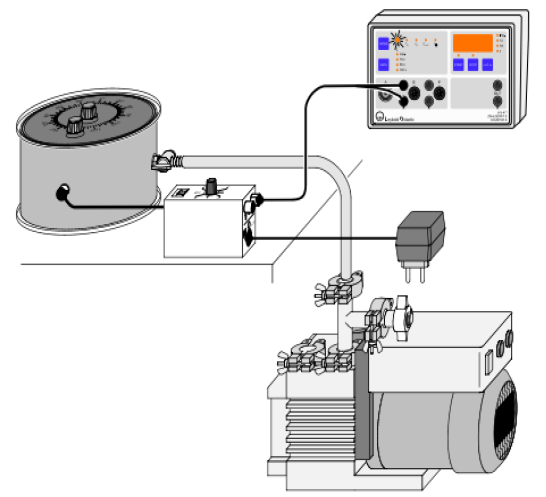
\includegraphics[width=0.8\columnwidth]{images/theory3.png}
			\caption{Experimental Setup}
			\label{fig:3}
		\end{figure}